% !TEX spellcheck = en-US
\documentclass[aps,prl,twocolumn,amsmath,amssymb,nobibnotes]{revtex4-1}%
\usepackage{graphicx}
\usepackage{dcolumn}
\usepackage{bm}
\usepackage{color}
\usepackage{amsmath}
\usepackage{epstopdf}
%\usepackage{caption}
%\usepackage{subcaption}
\usepackage{fancybox}
\usepackage{amsfonts}
\usepackage{amssymb}%
\usepackage[toc,page]{appendix}
\usepackage[symbol]{footmisc}
%\usepackage[backend=bibtex,natbib=true,sorting=none]{biblatex}
\setcounter{MaxMatrixCols}{30}


\renewcommand{\cite}[1]{{[}\onlinecite{#1}{]}}

\newcommand{\s}{\sum\limits}
\newcommand{\p}{\prod\limits}
\newcommand{\pa}{\partial}
\newcommand{\il}{\int\limits}
\newcommand{\be}{\begin{equation}}
\newcommand{\e}{\end{equation}}
\newcommand{\beml}{\begin{subequations}}
\newcommand{\eml}{\end{subequations}}
\newcommand{\beq}{\begin{eqnarray}}
\newcommand{\eq}{\end{eqnarray}}
\newcommand{\ba}{\begin{array}}
\newcommand{\ea}{\end{array}}
\newcommand{\bpm}{\begin{pmatrix}}
\newcommand{\epm}{\end{pmatrix}}
\newcommand{\bc}{\begin{cases}}
\newcommand{\ec}{\end{cases}}
\newcommand{\lt}{\left}
\newcommand{\rt}{\right}
\newcommand{\n}{\nonumber}
\newcommand{\la}{\langle}
\newcommand{\ra}{\rangle}
\newcommand{\ep}{\varepsilon}
\newcommand{\dd}{\displaystyle}
\newcommand{\bs}{\boldsymbol}
\newcommand{\h}{^\dagger}
\newcommand{\ph}{^{\phantom{\dagger}}}
\newcommand{\one}{\openone}
\newcommand{\ut}{\underaccent{\tilde}}
\newcommand{\ul}{\underaccent{\bar}}
\newcommand{\up}{\uparrow}
\newcommand{\dn}{\downarrow}
\DeclareMathOperator{\var}{var}
\DeclareMathOperator{\tr}{Tr}
\DeclareMathOperator{\diag}{diag}
\DeclareMathOperator{\im}{Im}
\DeclareMathOperator{\re}{Re}
\DeclareMathOperator{\ctg}{cotan}
\DeclareMathOperator{\arcsh}{arcsinh}
\DeclareMathOperator{\csch}{csch}
\DeclareMathOperator{\rot}{rot}

\newcommand{\AQ}[1]{\textbf{\textcolor{red}{{#1}}}}

\begin{document}
\title{Ultrafast Control of Spin-Spin Interactions in Two-Dimensional Magnetic Systems: Kane-Mele-Hubbard Model}

\author{Juan M. Losada}
\affiliation{Center for Quantum Spintronics, Department of Physics, Norwegian University of Science and Technology, NO-7491 Trondheim, Norway}
\author{Arne Brataas}
\affiliation{Center for Quantum Spintronics, Department of Physics, Norwegian University of Science and Technology, NO-7491 Trondheim, Norway}
\author{Alireza Qaiumzadeh}
\thanks{Corresponding author: alireza.qaiumzadeh@ntnu.no}
\affiliation{Center for Quantum Spintronics, Department of Physics, Norwegian University of Science and Technology, NO-7491 Trondheim, Norway}
%\affiliation{Institute for Advanced Studies in Basic Science (IASBS), Zanjan, Iran}

\begin{abstract}

\end{abstract}

\date{\today}
\maketitle




\textit{Model Hamiltoniantest}.---
Effective Hamiltonian of a 2D planar honeycomb lattice in the presence of electron-electron interactions can be described by Kane-Mele-Hubbard model \cite{Kane2005,Griset2012,Auerbach}. \AQ{cite papers for KMH model. Also cite Auerbach's book for Hubbard model!}
The Hamitlonian in the absence of external perturbations is the sum of the kinetic term $\hat{\mathcal{H}}_t$, the intrinsic SOI $\hat{\mathcal{H}}_{\text{SOI}}$ and electron-electron interaction modelled by extended Hubbard model $\hat{\mathcal{H}}_{\text{int}}$,
\begin{equation}
\label{MKMH}
\hat{H}_0 = \hat{\mathcal{H}}_{\text{K}} + \hat{\mathcal{H}}_{\text{SOI}} + \hat{\mathcal{H}}_{\text{int}},
\end{equation}
where
\begin{align}
\hat{\mathcal{H}}_{\text{K}} &= - \sum_{\langle i,j \rangle, \tau} t_{1}\hat{c}_{i \tau}^\dagger \hat{c}_{j \tau} - \sum_{\langle \langle i,j \rangle \rangle, \tau} t_{2}\hat{c}_{i \tau}^\dagger \hat{c}_{j \tau} \label{Ht} \\
\hat{\mathcal{H}}_{\text{SOI}} & = \sum_{\langle \langle i,j \rangle \rangle, \tau,\tau'} i\Delta\nu_{ij}\sigma^z_{\tau, \tau'}\hat{c}_{i \tau}^\dagger \hat{c}_{j \tau'} \label{Hsoi} \\
\hat{\mathcal{H}}_{\text{int}} &= U_{00}\sum_{i=1} \hat{n}_{i\uparrow}\hat{n}_{i\downarrow} + \frac{1}{2}\sum_{\langle i,j \rangle, \tau \tau'} V_{ij}\hat{n}_{i\tau}\hat{n}_{j\tau'} \label{Hint}.
\end{align}
\begin{figure}[t]
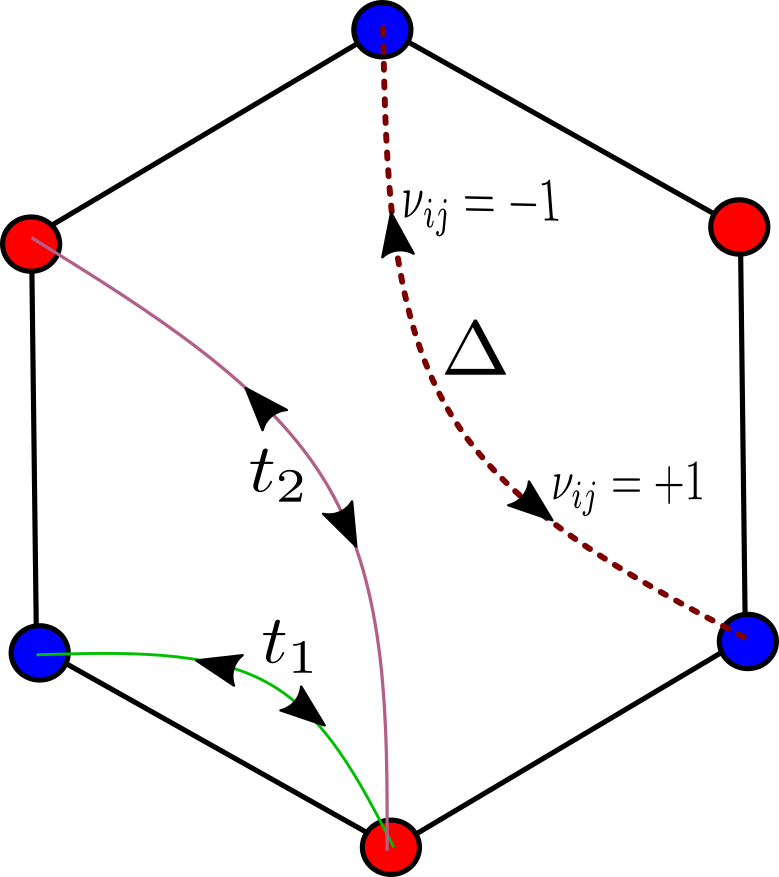
\includegraphics[width=0.6\columnwidth]{../Figures/kmh.png}
\caption{A honycomb cell with NN hopping $t_1$, NNN hopping $t_2$ and intrinsic SOI $\Delta$. $\nu_{ij} = \pm 1$ depending on whether the electron traversing from $i$ to $j$ makes a right ($+1$) or a left turn ($-1$).}
\label{fig1}
\vspace*{-6pt}
\end{figure}
where $\hat{c}_{i \sigma}^\dagger$ ($ \hat{c}_{i \sigma}$) are fermionic creation (annihilation) operators for an electron on site $i$ and spin state $\tau=\{\uparrow,\downarrow\}$, $t_1$ and $t_2$ are nearest-neighbour (nn) and  next-nearest-neighbour (nnn) hopping amplitudes, $\Delta$ is the intrinsic SOI constant, $\nu_{ij}=\pm 1$ depending on whether the electron traversing from $i$ to $j$ makes a right ($+1$) or a left turn ($-1$), $\sigma^{z}$ is the $z$-component of Pauli matrices $\bm{\sigma}$, $U_{00}$ and $V_{ij}$ are the on-site and nn Coulomb interactions.
The presence of the intrinsic SOI, Eq. (\ref{Hsoi}), reduces the $\mathrm{SU}(2)$ symmetry of a pure Hubbard model to the $\mathrm{U}(1)$ spin group.

Using the variational principle, it has been shown that the nn Coulomb interaction can be effectively approximated by a renormalized on-site interaction $U =U_{00} - \bar{V}$, where $\bar{V}$ is a weighted average of the nn Coulomb interaction \cite{Schuler2013,Stepanov2017}. Thus, we only take into account the local Coulomb interaction in our total Hamiltonian and rewrite the interaction part of the Hamiltonian (\ref{Hint}),
\begin{equation}
\hat{\mathcal{H}}_{\text{int}} \approx U\hat{d},
\end{equation}
where we define the doublon number operator $\hat{d} = \sum_{i=1} \hat{n}_{i\uparrow}\hat{n}_{i\downarrow}$ with eigenvalues $d$ and projection operators $\hat{P}_d$. We are interested to Kane-Mele-Hubbard model at half-filling in strong-coupling regime $U\gg t_{1(2)}$. In the strong-coupling limit any state with a nonzero number of double occupancies ($d \neq 0$) will have much larger energy than those with $d=0$. We obtain an effective Hamiltonian acting on the $d=0$ subspace by standard second-order perturbation theory in the hopping terms. Using the following relations,
\begin{align}
\hat{c}_{i \tau}^\dagger \hat{c}_{i \tau'} &= \frac{1}{2} (n_{i \uparrow} + n_{i \downarrow})\delta_{\tau \tau'}  + \bs{S}_i\cdot\bs{\tau}_{\tau', \tau}, \label{SpinOperatorInv1}\\
\hat{c}_{i \tau} \hat{c}_{i \tau'}^\dagger &= \frac{1}{2} (2 - n_{i \uparrow} - n_{i \downarrow}) \delta_{\tau \tau'} - \bs{S}_i\cdot\bs{\tau}_{\tau, \tau'}, \label{SpinOperatorInv2}
\end{align}
we find the spin Hamiltonian for 2D AFM Mott insulators,
\begin{align}
\label{MKMHeff0}
H_{\text{S}} =& J_{1}\sum_{\langle i,j \rangle} \bs{S}_i\cdot\bs{S}_j + J_{2}\sum_{\langle \langle i,j \rangle \rangle} \bs{S}_i\cdot\bs{S}_j\n \\
&+ \sum_{\langle \langle i,j \rangle \rangle} \bs{S}_i \bs{\Gamma}_{ij} \bs{S}_j +\sum_{\langle \langle i,j \rangle \rangle} \bs{D}_{ij}\cdot \bs{S}_i \times \bs{S}_j,
\end{align}
with the following spin-spin interactions,
\begin{align}
J_{1(2)} &= \frac{2t_{1(2)}^2}{U}, \\
\bs{\Gamma}_{ij} &=\frac{2\Delta^2}{U} \text{diag}(-1,-1,1),\\
\bs{D}_{ij} &= - \frac{4 t_2 \Delta}{U}\nu_{ij}  \hat{\mathrm{e}}_z.
\end{align}
The first and second terms in the spin Hamiltonian, Eq. (\ref{MKMHeff0}), are the nn and nnn symmetric Heisenberg AFM exchange interactions, $J_{1(2)}>0$, respectively; the third term is a nnn Heisenberg XXZ-like term arising from the intrinsic SOI, and finally, the last term is the intrinsic nnn DMI. The intrinsic SOI in Eq. (\ref{Hsoi}), leads to a DMI vector, $\bs{D}_{ij}$, perpendicular to the honeycomb plane while it is straightforward to show that the Rashba SOI, arising from breaking the inversion symmetry of the honeycomb lattice, results an inplane DMI vector perpendicular to the lattice bonds.
For the sake of completeness, we explain shortly the effect of disorders by adding an on-site disorder $\sum_{i \tau} \varepsilon_i \hat{c}_{i \tau}^\dagger \hat{c}_{i \tau}$ in the Kane-Mele-Hubbard Hamiltonian \ref{MKMH}, where $\varepsilon_i$ is an uncorrelated random variable. Following the above procedure, it can be shown that the spin interaction parameters are only renormalized by $U^{-1} \rightarrow U/\left(U^2-(\epsilon_j-\epsilon_i)^2\right)$ \cite{Protopopov2018}. In the large $U$ limit, the effect of disorder is negligible and we thus ignore it in the rest of this Letter.


Different terms appeared in the spin Hamiltonian derived in Eq. (\ref{MKMHeff0}) has already been obtained phenomenologically in several  \cite{Owerre2016} and confirmed experimentally \cite{Chen2018} but, to the best of our knowledge, this is the first microscopic derivation of the complete spin Hamiltonian $\hat{H}_{\text{S}}$ from the Kane-Mele-Hubbard model.
It has been shown that this Hamiltonian has interesting features and exotic phases like, existence of magnon spin Nernst effect in collinear AFM layers \cite{Cheng2016, Zyuzin2018} \AQ{cite two PRLs by Ran Cheng and Alexy Kovalev}, topological magnon insulator phase \cite{Owerre2016, Elyasi2018, Chen2018}, spin Hall effects of Weyl magnons \cite{Zyuzin2018, Sekine2016} magnonic Floquet topological insulators, spin density wave \cite{Mulder2010}, chiral and topological gapped spin liquid phases \cite{Vaezi}.



\textit{Laser illumination}. The effect of laser irradiation on the honeycomb lattice is introduced in the Kane-Mele-Hubbard Hamiltonian, Eq. (\ref{MKMH}), via the Peierls substitution method \cite{Peierls1933}. \AQ{cite to Pierls paper in Z Physics} The electric-field component of a polarized laser pulse is given by $\bs{E}(t) = \frac{E_0}{2}( e^{-i\omega t}\hat{\epsilon}+\mathrm{c.c.})$, where $E_0$ is the electric field amplitude, $\omega$ is the laser pulse frequency, and $\hat{\epsilon} = (\hat{\mathrm{e}}_x+i\lambda\hat{\mathrm{e}}_y)/\sqrt{1+\lambda^2}$ is the polarization unit vector with $\lambda= 0$ for linear polarization and $\lambda= \pm 1$ for right- and left handed polarizations.

It is more convenient to rewrite the noninteracting part of the Kane-Mele-Hubbard Hamiltonian, Eq. (\ref{MKMH}), from now on the hopping part, as $\hat{T}_0=\hat{\mathcal{H}}_{\text{K}}+\hat{\mathcal{H}}_{\text{SOI}} = - \sum_{i,j , \tau, \tau'}
t_{ij}^{\tau\tau'} \hat{c}_{i \tau}^\dagger \hat{c}_{j \tau'}$, where the hopping amplitude is $t_{ij}^{\tau\tau'} = \delta_{\tau,\tau'}t_1$ for $i,j$ being nn and $t_{ij}^{\tau\tau'} = \delta_{\tau,\tau'}t_2 - i\Delta\nu_{ij}\sigma^z_{\tau, \tau'}$ for $i,j$ being nnn.
According to the Peierls substitution method, the hopping part of the Hamiltonian in the presence of electromagnetic fields gain an extra phase $t_{ij}^{\tau\tau'}\rightarrow t_{ij}^{\tau\tau'} e^{{i e \bs{R}_{ij} \cdot \bs{A}(t)}/\hbar}$, where $\bs{R}_{ij} = \bs{R}_i-\bs{R}_j$, $\bs{R}_i$ is the position of site $i$, $e$ is the electronic charge, $\hbar$ is the reduced Planck constant, and $\bs{A}$ is the vector potential of laser pulse $\bs{A}(t) = \frac{1}{2}(\bs{A} e^{-i\omega t} + \mathrm{c.c.})$, with $\bs{A} = \frac{iE_0}{\omega}\hat{\epsilon}$.
The argument of the Peierls phase can be rewritten as $e\bs{R}_{ij}\cdot\bs{A}/\hbar \equiv \alpha_{ij} e^{i \theta_{ij}}$, with $\alpha_{ij} = \pm|e\bs{R}_{ij}\cdot \bs{A}|/\hbar$, in a such way that $\alpha_{ij}= -\alpha_{ji}$, $\theta_{ij}= \theta_{ji}$, and $\theta_{ij} \in \left[0,\pi\right)$.
Now, we use the Jacobi–-Anger expansion to rewrite the Peierls phase in the basis of its harmonics,
\begin{equation}
\label{JacobiAnger}
e^{i\frac{e}{\hbar}\bs{R}_{ij}\cdot\bs{A}(t)} = \sum_m e^{i(\frac{\pi}{2}-\theta_{ij})m} \mathcal{J}_m(\alpha_{ij}) e^{im\omega t}
\end{equation}
where $\mathcal{J}_m(x)$ is the \textit{m}-th Bessel function of the first kind \cite{Kitamura2017}.

The total Hamiltonian in the presence of the laser field is time depended through its hopping part, $\hat{H}(t) = \hat{T}(t) +  U\hat{d}$. Using Eq. (\ref{JacobiAnger}), we find $\hat{T}(t) = \sum_m \hat{T}_m e^{im \omega t}$, where $\hat{T}_m$ is the sum of all the \textit{m}-th Fourier mode of the hopping terms. Finally, we decompose the hopping operator into,
\begin{equation}
\hat{T}(t) = \sum_m (\hat{T}_{-1,m}+\hat{T}_{0,m}+\hat{T}_{1,m})e^{im\omega t},
\end{equation}
where $\hat{T}_{dm}(t)$ changes the doublon number by $d$, for example, if $\hat{P}_d$ is the projection operator into the subspace with doublon number $d$, then $\hat{T}_{dm}(t) = \sum_i \hat{P}_{i+d}\hat{T}_{m}(t)\hat{P}_i$.

To find the renormalized spin Hamiltonian, first, we have to find an effective time-independent Hamiltonian. To do that, we transform the original time-dependent Hamiltonian, $\hat{H}(t)$, using a unitary transformation $\hat{U}(t) = e^{-i\hat{S}(t)}$,
\begin{equation}
\hat{H}'(t) = e^{i\hat{S}(t)} \left(\hat{H}(t)  -  i\partial_t \right) e^{-i\hat{S}(t)}.
\label{Htransformed}
\end{equation}
We perform the unitary transformation perturbatively in the hopping parameter. We can formally write $\hat{T}(t) = \eta \hat{T}(t)$, where $\eta$ play the role of a bookkeeping parameter in the perturbation expansion. We expand $\hat{S}(t) = \sum_\nu \eta^\nu \hat{S}^{(\nu)}(t)$ and $\hat{H}'(t) = \sum_\nu \eta^\nu \hat{H}'^{(\nu)}(t)$. Our demand is that the transformed Hamiltonian must have the same periodicity of the original time-dependent Hamiltonian thus the unitary transformation itself must have the same periodicity of the driven laser field so that $\hat{S}^{(\nu)}(t) = \sum_m e^{im\omega t}\hat{S}^{(\nu)}_m$. Additionally, we impose that the transformed Hamiltonian to be block diagonal in the doublon number $d$ while $\hat{S}(t)$ does not contain block-diagonal terms. With these conditions the unitary transformation might be uniquely determined,
\begin{equation}
\hat{S}^{(\nu)}(t) = \sum_{d \neq 0} \sum_m \eta^\nu \hat{S}^{(\nu)}_{d,m} e^{im\omega t}
\end{equation}
where $\hat{S}^{(\nu)}_{d,m}$ changes the double occupancy number by $d$. We expand the transformed Hamiltonian \ref{Htransformed} in power series of $\eta$ and determine $\hat{S}^{(\nu)}(t)$ iteratively in $\nu$ so that $\hat{H}'^{(\nu)}(t)$ is diagonal in the doublon number. After tedious but straightforward calculations, the transformed Hamiltonian up to the second order in the hopping parameter is obtained $\hat{H}'(t)= \hat{T}'(t)+\text{U}\hat{d}$, where
\begin{align}
\label{transformedH}
\hat{T}'(t) \approx & - \sum_m \hat{T}_{0,m}(t)e^{im\omega t} + \n \\
&+ \frac{1}{2}\sum_{mn} \left( \frac{\left[\hat{T}_{1,n}, \hat{T}_{-1,m-n} \right]}{\text{U}+n\omega} - \frac{\left[\hat{T}_{-1,n}, \hat{T}_{1,m-n} \right]}{\text{U}-n\omega} \right) e^{im\omega t}.
\end{align}
Now, we are in the situation that we can calculate the effective time-independent Hamiltonian by time averaging of the transformed Hamiltonian $\hat{H}_{\text{eff}}=\hat{P}_0\hat{H}'(t)\hat{P}_0$, where $\hat{P}_0$ is the projection operator to the $d=0$ subspace.
Doing some algebra, the effective time-independent Hamiltonian in terms of creation and annihilation operators is obtained,
\begin{align}
\hat{H}_{\text{eff}} &= - \sum_{i,j, \tau, \tau'} \left(t_{ij}^{\tau} t_{ji}^{\tau'} \sum_{n} \frac{\mathcal{J}_{n}^2(\alpha_{ij})}{\text{U}+n\omega} \right)  \hat{c}_{i \tau}^\dagger \hat{c}_{j \tau} \hat{c}_{j \tau'}^\dagger \hat{c}_{i \tau'}+\text{U}\hat{d}. \label{GeneralHeff}
\end{align}


Finally, the spin Hamiltonian, at half-filling and strong interaction limit of the effective Hamiltonian $\hat{H}_{\text{eff}}$, using the relations Eqs. (\ref{SpinOperatorInv1}) and (\ref{SpinOperatorInv2}), is given by,
\begin{align}
\label{MKMHeffw}
\tilde{H}_{\text{S}}(\omega) =& \tilde{J}_{1}\sum_{\langle i,j \rangle} \bs{S}_i\cdot\bs{S}_j + \tilde{J}_{2}\sum_{\langle \langle i,j \rangle \rangle} \bs{S}_i\cdot\bs{S}_j\n \\
&+ \sum_{\langle \langle i,j \rangle \rangle} \bs{S}_i \tilde{\bs{\Gamma}}_{ij} \bs{S}_j +\sum_{\langle \langle i,j \rangle \rangle} \tilde{\bs{D}}_{ij}\cdot \bs{S}_i \times \bs{S}_j,
\end{align}
with the following renormalized spin interactions,
\begin{align}
\label{Renor-para}
\tilde{J}_{1,ij} &= 2t_1^2\frac{\mathcal{J}_{n}^2(\alpha_{ij})}{\text{U}+n\omega}, \\
\tilde{J}_{2,ij} &= 2t_2^2\frac{\mathcal{J}_{n}^2(\alpha_{ij})}{\text{U}+n\omega}, \\
\tilde{\bs{D}}_{ij} &= - 4 t_2 \Delta \frac{\mathcal{J}_{n}^2(\alpha_{ij})}{\text{U}+n\omega} \nu_{ij} \hat{\mathrm{e}}_z, \\
\tilde{\bs{\Gamma}}_{ij} &= 2\Delta^2 \text{diag}(-1,-1,1) \frac{\mathcal{J}_{n}^2(\alpha_{ij})}{\text{U}+n\omega}.
\end{align}
All spin interaction parameters are renormalized by the same function but $\alpha_{ij}$ is different for nn and nnn parameters which is peculiar of honeycomb lattices described by the Kane-Mele-Hubbard model. Thus, the ratios between these renormalized parameters are different than non-perturbed parameters. The renormalized spin interactions presented in Eq. \ref{Renor-para} are independent from helicity of laser pulse and are the same for both circular and linear polarizations.


\begin{figure}[t]
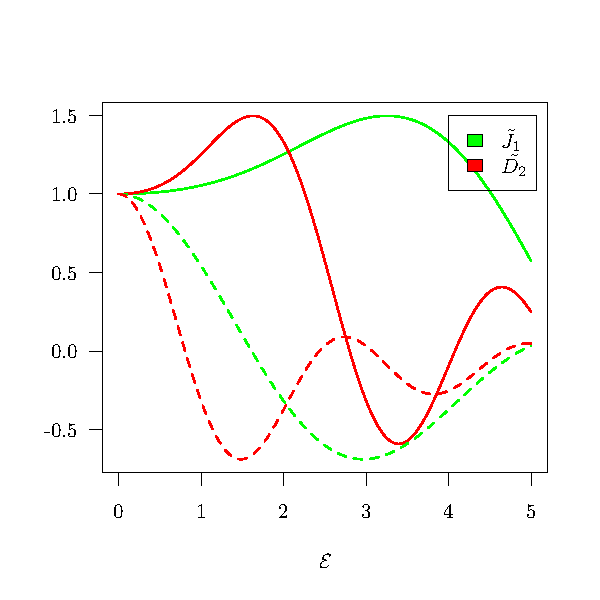
\includegraphics[width=\columnwidth]{../Figures/NNvsNNN.pdf}
\caption{For circularly polarized light we obtain $\tilde{J}_1 = \frac{J_{1,ij}'}{J_{1,ij}}$ and $\tilde{D}_{2} = \frac{D_{2,ij}'}{D_{2,ij}}$ as function of $\mathcal{E} = \frac{eaE_0}{\omega}$. Solid lines are for $\omega = 4$ and dashed lines are for $\omega = 14$. Notice that $\tilde{J}_1$ and $\tilde{D}_{2}$ do not depend on the parameters $t_1$, $t_2$ and $\Delta$.}
\label{fig2}
\vspace*{-6pt}
\end{figure}


Figure \ref{fig2}, shows the dependence of normalized nn exchange interaction $\tilde{J}_{1,ij}/J_{1,ij}$ and normalized nnn DMI $\tilde{D}_{ij}/D_{ij}$ in the dimensionless electric field parameter $\mathcal{E} = \frac{e a E_0}{\omega}$, where $a$ is the lattice constant. The results are obtained for dimensionless material parameters $t_1=1$, $\text{U} = 10$ and $\omega = 4 \mathrm{and} 14$ (equivalently, $T = \frac{2\pi}{\omega} \approx 10^{-16}\text{s}$). Figure \ref{fig2}, shows that it is possible not only change the sign and amplitude of the exchange interaction as already reported in Ref. \cite{Mentink2015} but its is possible to change the signa nd amplitude of intrinsic DMI. More importantly, the ratio $\tilde{J}_{1,ij}/\tilde{D}_{ij}\neq J_{1,ij}/D_{ij}$ can be tuned by laser excitations which is responsible for ultarafast photoinduced spin dynamics and magnon scattering phenomena.

Eqs. (\ref{MKMHeffw}) and (\ref{Renor-para}) explicitly show that the spin Hamiltonian in the presence of a time-dependent external field can be effectively written as $\tilde{H}_{\text{S}}=H_{\text{S}}+g_{\alpha \beta i j} S^\alpha_i S^\beta_j E^{\alpha} E^{*\beta} $, where $\alpha$ and $\beta$ stand for spatial component of vectors, and $i$ and $j$ refer to the lattice cite. Thus, the dielectric permittivity tensor is given by $\varepsilon_{\alpha \beta}=\partial^2 \tilde{H}_{\text{S}}/\partial E^{\alpha}\partial E^{*\beta}$, where $g$ is the response function tensor. This optomagnetic effect described by the dielectric permittivity $\varepsilon$, can be detected by measuring the intensity of the scattered light $I_{\mathrm{sc}} \propto (\varepsilon_{\alpha \beta} E_0)^2$ \cite{Demokritov1985}.

In ultrafast spin dynamics experiments, very intense laser pulses are used and one might think about heating and concerning on the validity of our approach. Recent theoretical \cite{Rudner2019} and experimental \cite{PhysRevA.96.053602} works show that the energy absorption rate is suppressed exponentially for high frequency laser pulses $\omega/W\gg 1$, where $W\propto t_1$ is the fermionic bandwidth, which is the case in ultrafast experiments with optical laser pulses. Thus, rapidly driven systems have a very long prethermalization period and this implies that the evolution of these systems in the presence of short laser pulses can be described by our formalism safely.



There are some recent experiments on possibility of ultrafast optical modification of exchange interactions in the bulk of iron oxides \cite{Mikhaylovskiy2015,Kim2016,Jin2014} \AQ{cite to Nature Communications volume 6, Article number: 8190 (2015)and find similar papers}. We hope that our work stimulate new experiments on measuring exchange interaction and DMI in 2D magnetic systems.


\section*{Acknowledgments}
The research leading to these results was supported by the European Research Council via Advanced Grant No. 669442, ``Insulatronics,'' and by the Research Council of Norway through its Centres of Excellence funding scheme, Project No. 262633, ``QuSpin.''


%\begin{thebibliography}
\bibliographystyle{apsrev4-1}
\bibliography{paper}
%\end{thebibliography}

\end{document}


